\section*{10. Multi-Layer Perceptrons}
\begin{figure}[H]
    \centering
    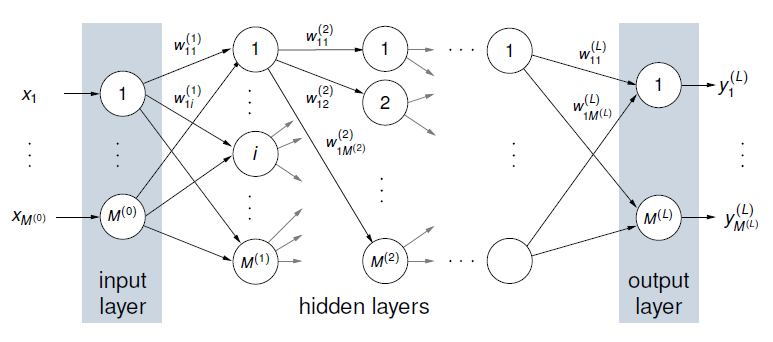
\includegraphics[scale=0.6]{figures/nn}
\end{figure}
\begin{itemize}
    \item
        Output value $y_j^{(l)}$ of $j$-th perceptron at layer $l$ is calculated by weighting up the outputs of perceptrons of the previous layer and subtracting a bias. The so calculated value then gets fed into an activation function (e.g. sigmoid function)
        \begin{align*}
            &net_j^{(l)} = \sum_{i=1}^{M^{(l-1)}} y_i^{(l-1)}w_{ij}^{(l)} - w_{0j}^{(l)}
            &y_j^{(l)} = f(net_j^{(l)})
        \end{align*}
\end{itemize}
\subsection*{Backpropagation \footnote{http://neuralnetworksanddeeplearning.com/chap2.html}}
\begin{itemize}
    \item
        Notation:
        \begin{itemize}
            \item
                $w_{jk}^l$ (weight for the connection from $k$-th neuron in $(l-1)$-th layer to $j$-th neuron), $b_j^l$ (bias)
            \item
                $C = \ffrac{1}{2} \norm{y-a^L}^2$ (Mean square error cost function of one training example)
            \item
                $\nabla_a C$ (vector expressing rate of change of $C$ with respect to the output activation)
            \item
                $\odot$ (elementwise vector multiplication, Hadmard product)
            \item
                $a_j^l = \sigma(\sum_k w_{jk}^l a_k^{l-1} + b_j^l)$ (output of neuron)
            \item
                $z_j^l = \sum_k w_{jk} a_k^{l-1} + b_j^l$ (weighted input without activation)
        \end{itemize}

    \item
        Key equations:
        \begin{enumerate}
            \item
                $\delta^L = \nabla_a C \odot \sigma'(z^L)$
            \item
                $\delta^l = ((w^{l+1})^T \delta^{l+1})\odot \sigma'(z^l)$
            \item
                $\ffrac{\partial C}{\partial b_j^l} = \delta_j^l$
            \item
                $\ffrac{\partial C}{\partial w_{jk}^l} = a_k^{l-1} \delta_j^l$
        \end{enumerate}

    \item
        Explanation:
        \begin{itemize}
            \item
                Goal: Compute $\partial C/\partial w_{jk}^l$ and $\partial C/\partial b_j^l$ and do parameter tuning via gradient descent
            \item
                To compute those, we first introduce an intermediate quantity $\delta_j^l$, which we call error 
            \item
                $\delta_j^l \equiv \ffrac{\partial C}{\partial z_j^l}$. "Partial derivative of cost function with respect to weighted sum neurons input"
            %\item
            %    1) $\ffrac{\partial C}{\partial a_j^L}$: "How fast does cost change as a function of activation". $\sigma'(z_j^L)$: "How fast does activation change at $z_j^L$"
            %\item
            %    2): Moves error backword through the activation function
            %\item
            %    3) 4): Now let's us compute partial derivatives of weights and bias
        \end{itemize}
    \item
        Algorithm:
        \begin{enumerate}
            \item
                Input $x$: Set the corresponding activation $a^1$ for the input layer
            \item
                Feedforward: For each $l = 2,3,\dots,L$ compute $z^l = w^l a^{l-1} + b^l$ and $a^l = \sigma(z^l)$
            \item
                Output error $\delta^L$: Compute the vector $\delta^L = \nabla_a C \odot \sigma'(z^L)$
            \item
                Backpropagate the error: For each $l = L-1, L-2, \dots, 2$ compute $\delta^l$
            \item
                Output: Gradient of cost function w.r.t weights and biases
        \end{enumerate}
    \item
        Update rule: $\Delta w_{ij}^{(l)} = -\eta \ffrac{\partial C}{\partial w_{ij}^{(l)}} = \eta \delta_j^{(l)}a_i^{(l-1)}$, where $\eta$ is the learning rate
    \item
        Intuition behind error $\delta$
        \begin{itemize}
            \item
                Last layer perceptrons want to know, how they have to adjust its output values in order to improve classification results
            \item
                The layer before also wants to know, how it's output values have to be adjusted and so on (this obviously depends on the cost improving outputs of the next layer) $\rightarrow$ backpropagation
            \item
                With the error informations at hand, the weight and bias gradients can be calculated
            \item
                Via gradient descent the parameter values then get improved
        \end{itemize}
\end{itemize}
